\section{Revis\~ao da Literatura}\label{sec:refteo}

Este capítulo apresenta uma revisão sistemática  da literatura (RSL) nos temas relacionados a previsão de séries temporais e aplicações em hidrologia e mais especificamente em abastecimento d'água. A revisão bibliográfica realizada consiste em uma análise abrangente e crítica das principais fontes de literatura. As informações extraídas da literatura são fundamentais para embasar a fundamentação teórica, a metodologia e a análise dos resultados deste estudo.


A seleção das referências foi baseada em critérios específicos tais como. Definição das bases de busca, escolha das \textit{keywords}, seleção do período de busca ($2016$ a $2024$), seleção do tipo de artigo, organização pela ordem de citações, verificação dos periódicos mais importantes (fator Q1 do Scimago e Fator de Impacto (FI)). Se um periódico pertencer ao quartil Q1 do Scimago significa que tem um desempenho melhor do que pelo menos $75$\% das revistas dessa mesma categoria. Embora nem todas as referências obtidas tenham uma relação evidente ou mesmo acentuada com a área de aprendizado de máquina, elas contribuem como material de suporte a implementação de alguns modelos avaliados para previsão nesta dissertação e podem servir como base para outros estudos.

A Figura \ref{fig:serie-temporal} apresenta um fluxograma de como a pesquisa foi realizada, destacando a importância da escolha dos periódicos Q1 e com maior fator de impacto, como base para esta RSL. A mesma figura apresenta uma adaptação da metodologia proposta por \citeonline{MARTINS201671} para a realização da RSL, onde primeiramente foram realizadas buscas na base Scopus e \textit{Web of Science} (WoS), selecionando referências relevantes para o tema da pesquisa. Para as duas bases de busca utilizadas foram usadas as palavras-chave ``\textit{time series forecasting}'', ``\textit{time series analysis}'', ``\textit{sanitation}'' e ``\textit{water supply}'' .

\begin{figure}[!htb]
	\centering
	\caption{Fluxograma da Revisão Sistemática da Literatura.}
	\label{fig:serie-temporal}
	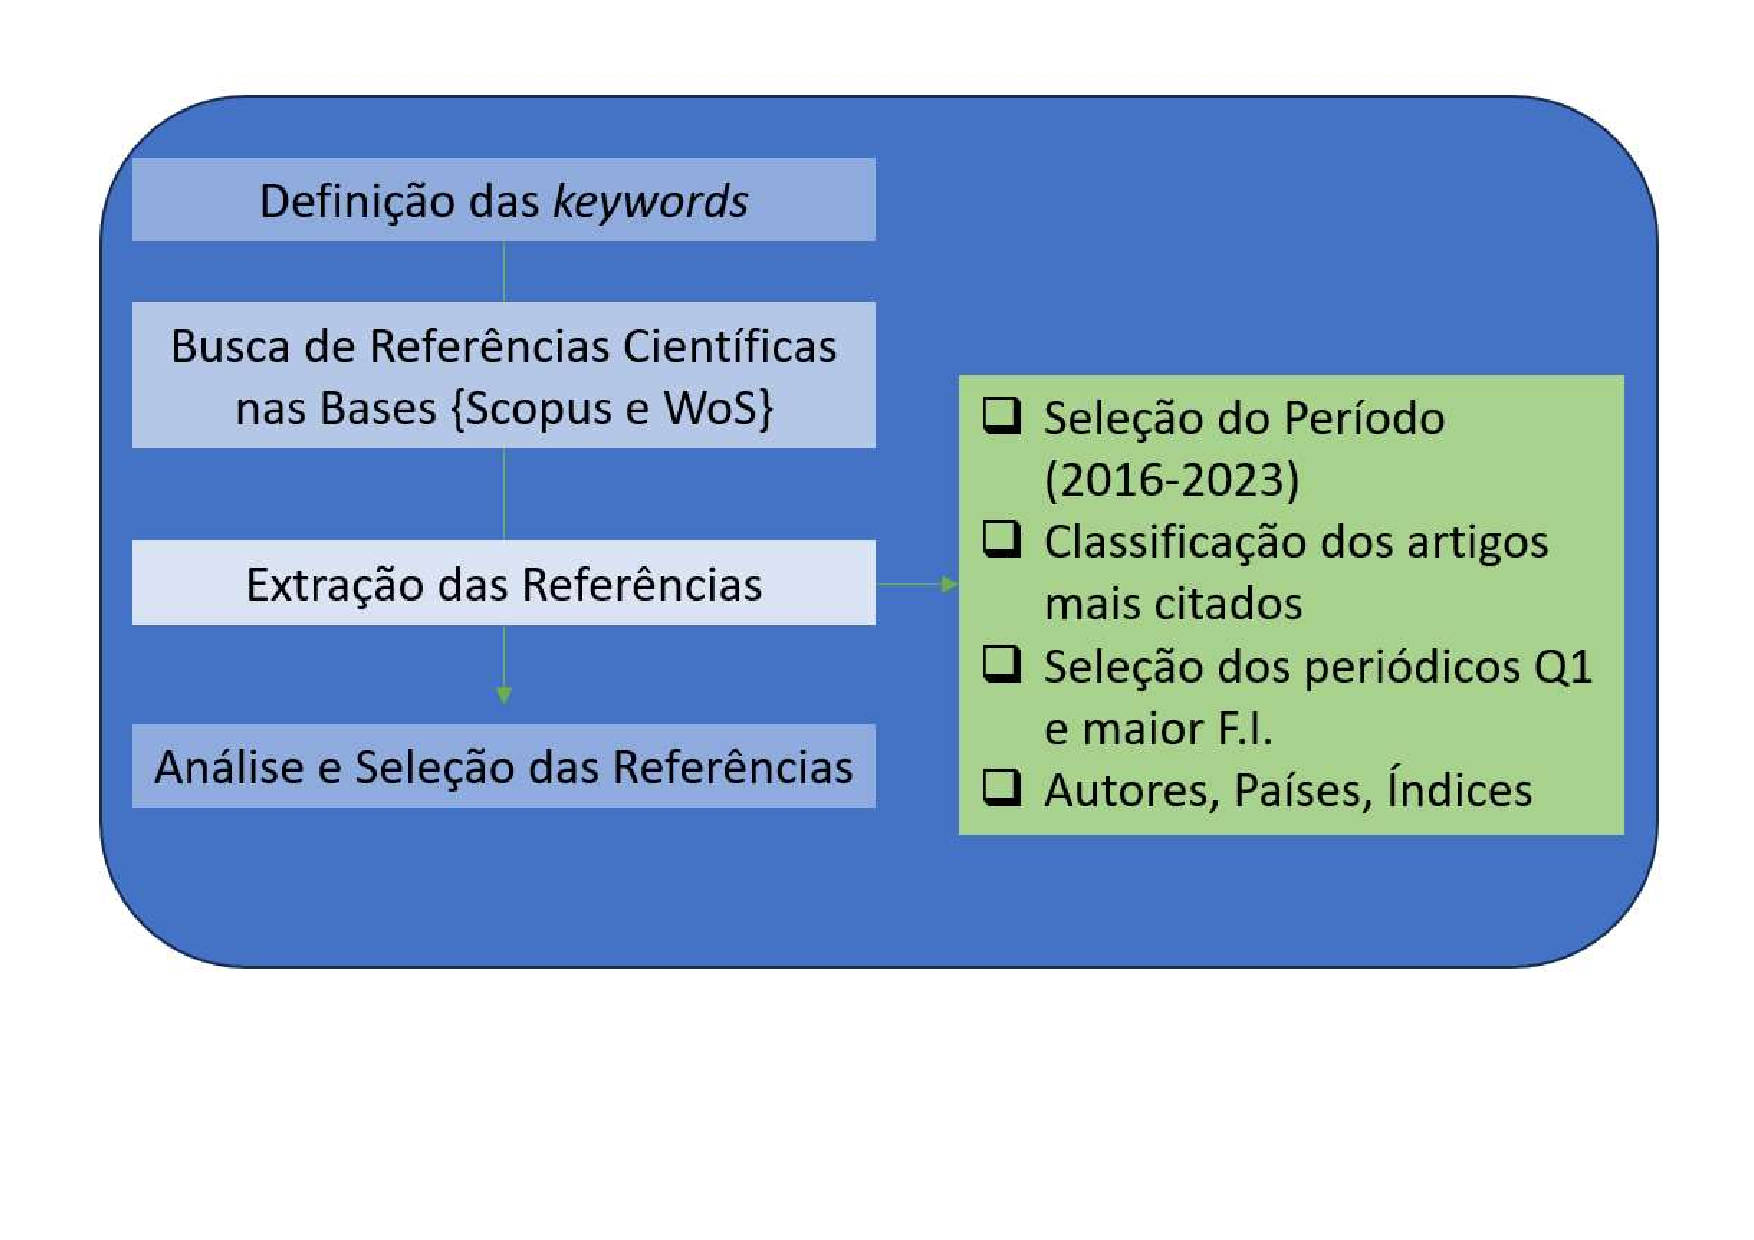
\includegraphics[width=0.7\linewidth]{Revisao/Figuras/Figura2.pdf}
\end{figure}

Na etapa seguinte, foi realizada uma avaliação preliminar de cada artigo obtido.

\noindent\textbf{Critérios de Inclusão}:

\begin{enumerate}
	\item Idioma: Os artigos considerados devem estar escritos em inglês.
	\item Tipo de Publicação: Devem ser artigos (\textit{papers}).
	\item Base de Dados: Artigos provenientes de bases de dados como Scopus e WoS são considerados.
\end{enumerate}

\noindent\textbf{Critérios de Exclusão}:

\begin{enumerate}
	\item Filtro Anual: de $2016$ a $2024$.
	\item Duplicatas: Artigos duplicados serão removidos durante o processo de revisão.
	\item Número Elevado de Artigos: Diante da quantidade significativa de artigos encontrados, optou-se por realizar uma análise preliminar sem a aplicação de filtros anuais para otimizar o processo de busca. Na base de dados Scopus, por exemplo, existiam $831$ artigos, enquanto na base de dados WoS, foram encontrados 98 artigos, totalizando $929$ artigos.
\end{enumerate}


Levando em consideração a diferença entre essa estimativa apresentada na Tabela \ref{tab:resumo} e a quantidade de artigos restantes após a remoção de duplicatas, tem-se menos de $929$ artigos para análise. É válido lembrar que, ao remover as duplicatas, o número diminuiu ainda mais, chegando a 906 artigos.

Na etapa final, foi realizada uma análise dos conteúdos dos artigos selecionados, levando em consideração as áreas de especialização. Como esta revisão está inserida no contexto de um programa de mestrado em Engenharia de Produção e Sistemas, vale a pena analisar a relação dos artigos obtidos com áreas afins como Matemática. Assim, as áreas mais relevantes para a pesquisa foram Informática, Engenharia e Matemática, representando $50\%$ das publicações. 

São apresentados os resultados da RSL, utilizando um \textit{software} VOSviewer de cada base de dados utilizada no trabalho. 
A Figura \ref{fig:scopus-09-08} mostra os modelos de previsão usados com frequência em conjunto com ``\textit{time series}'' nos artigos obtidos nas bases de dados Scopus e WoS. 

\begin{figure}[!htb]
	\centering
	\caption{Modelos de previsão de series temporais na base de dados Scopus e WoS.}
	\label{fig:scopus-09-08}
	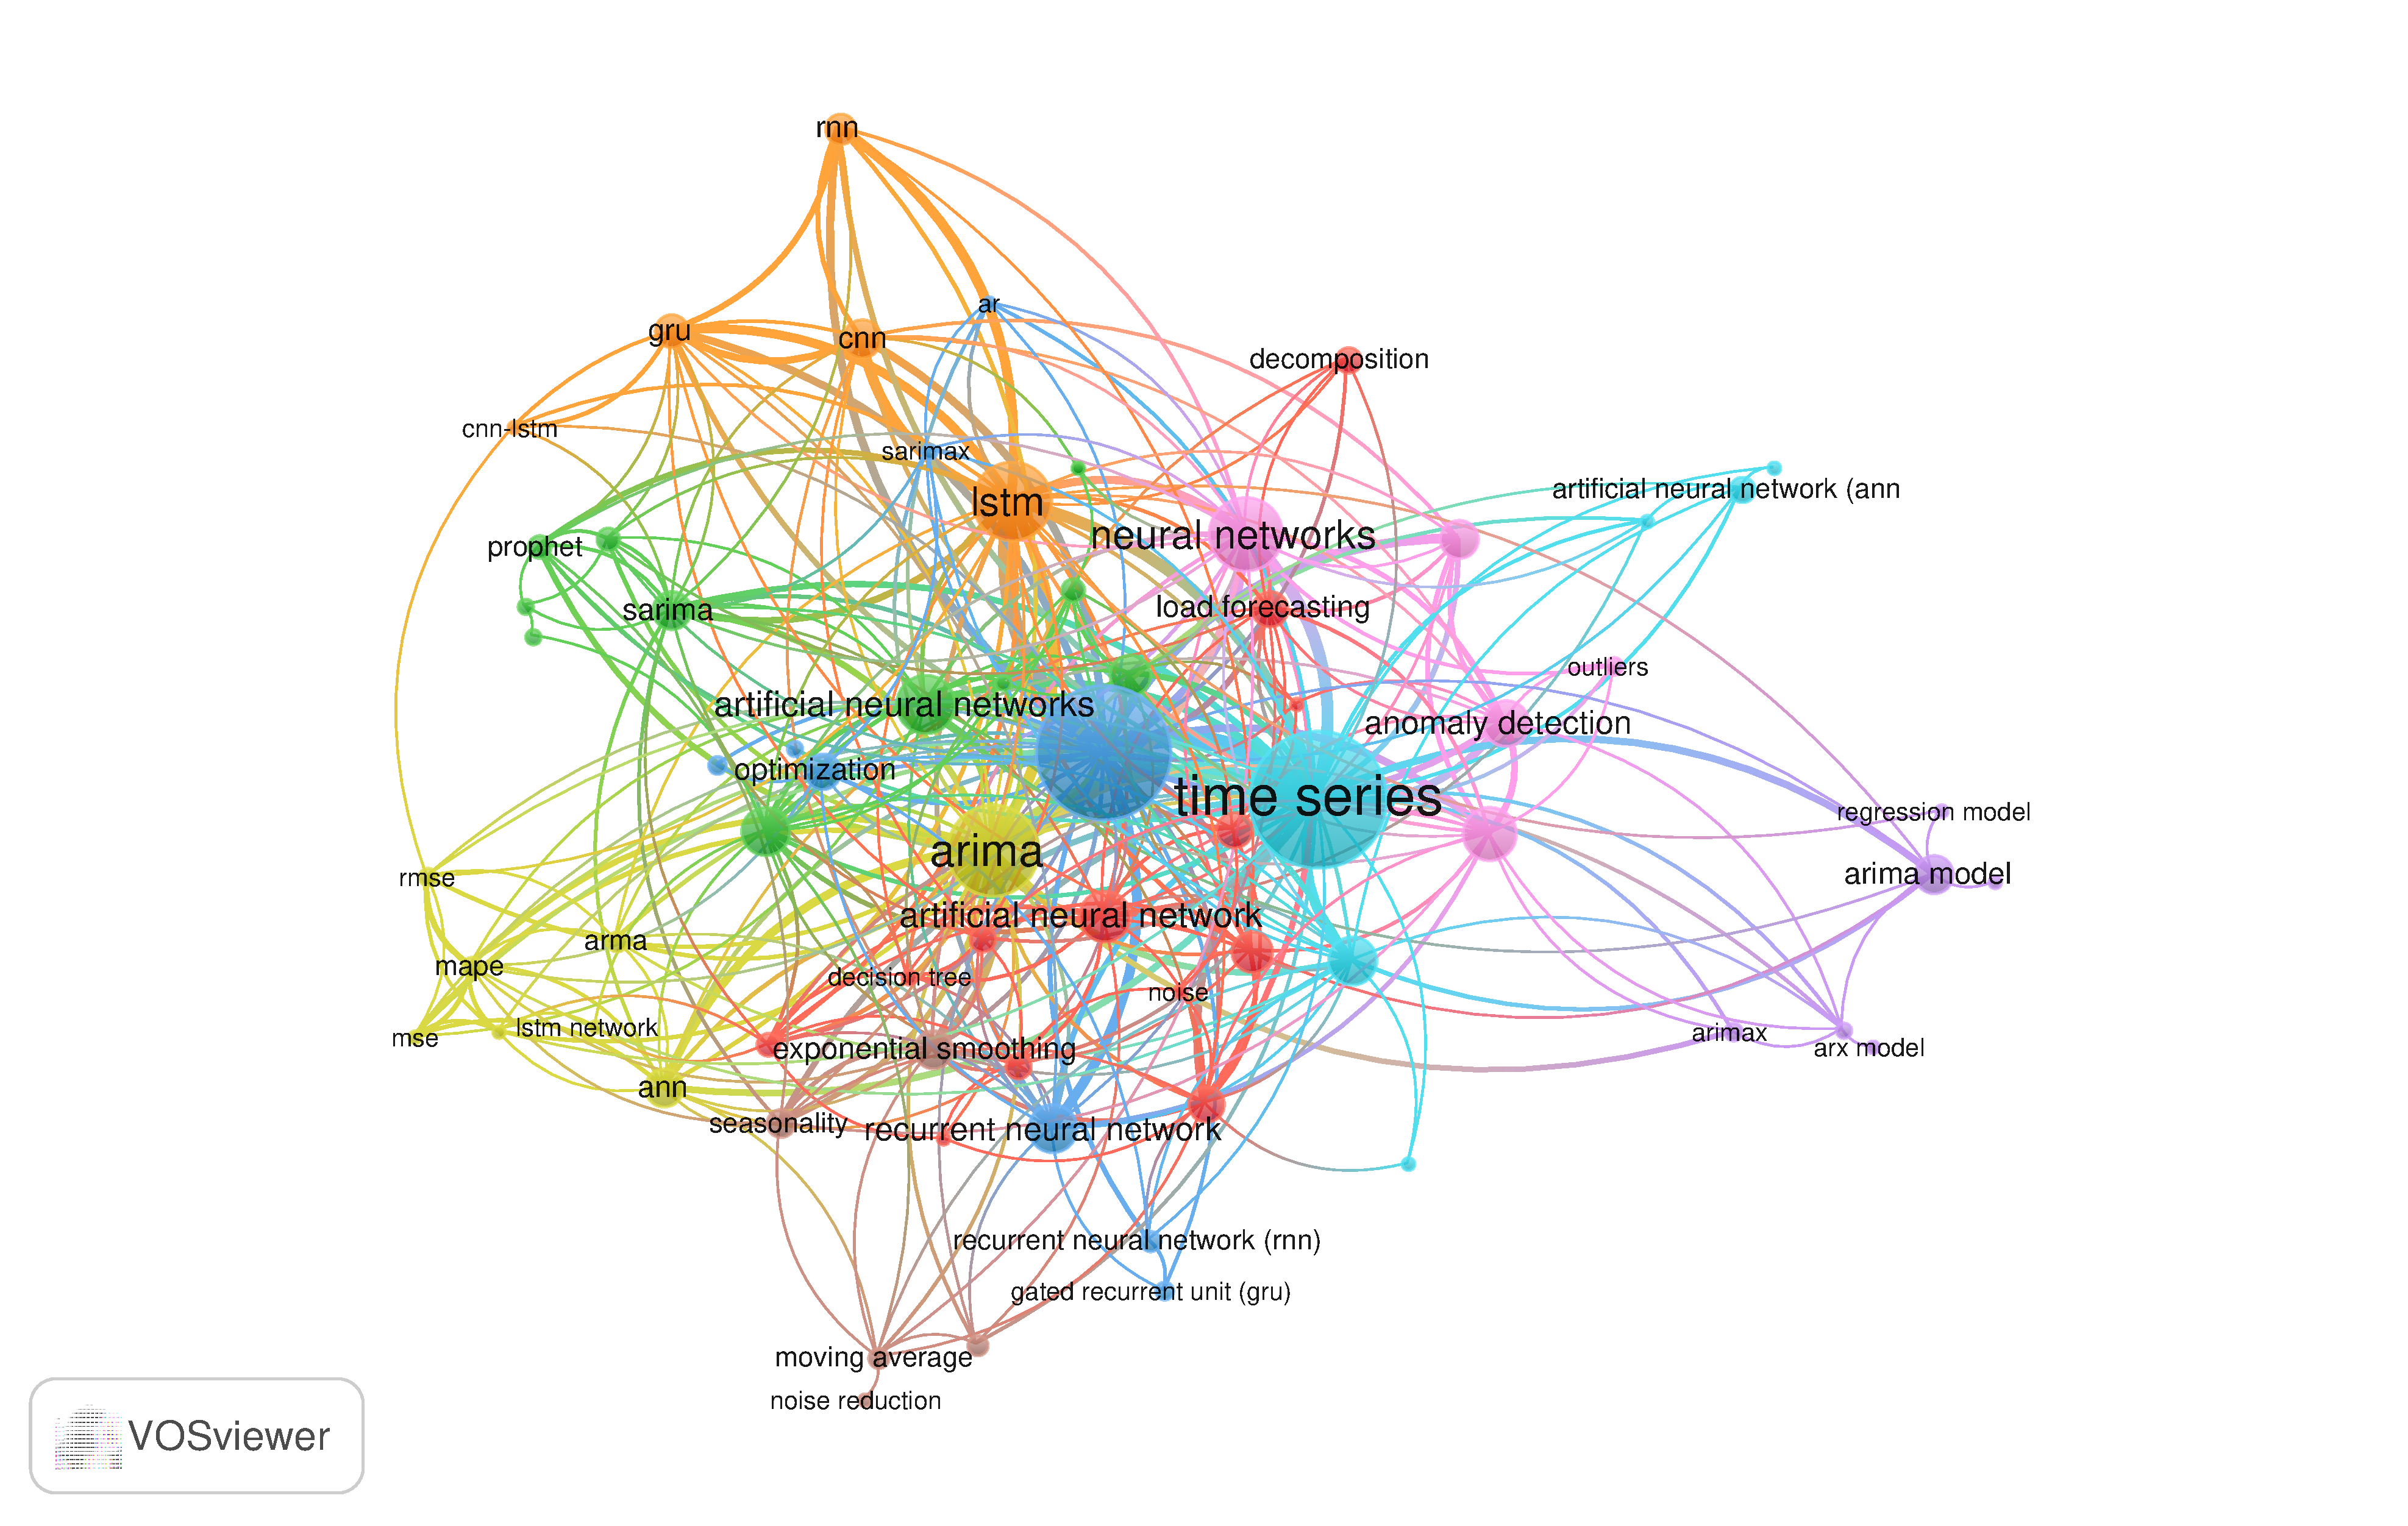
\includegraphics[width=\linewidth]{Revisao/Figuras/base-wos-scopus.pdf}
	
	
\end{figure}

Nesse primeiro momento, foram obtidos $2.555$ modelos, dos quais $83$ modelos são dispostos na Figura \ref{fig:scopus-09-08}. É importante destacar que as palavras-chave utilizadas foram \textit{time series forecasting} ou \textit{time series analysis} e \textit{water supply} e \textit{sanitation} em ambas as bases de dados. Os modelos apresentados na Figura \ref{fig:scopus-09-08} têm como base para as escolhas os modelos mais utilizados na literatura. Com essa visão mais geral, é possível ter um ponto de partida para a escolha dos modelos.

A Tabela \ref{tb1} apresenta as palavras-chave utilizadas em cada base de dados, juntamente com o número de artigos obtidos. No entanto, é importante ressaltar que esses dados ainda não foram processados para remover dados duplicados. Após, foi utilizado o software \textit{ScientoPy} para eliminar artigos repetidos, foram selecionados então $308$ artigos. Esses artigos foram analisados na RSL e são considerados relevantes para este estudo. Na primeira análise das bases de dados, foram relacionadas duas palavras-chave importantes, que são \textit{time series forecasting} e \textit{time series analysis}, apenas para ter a dimensão dos dados que estão sendo trabalhados tanto na Scopus quanto na WoS. Cada uma retornou valores distintos, e ao relacionar as mesmas palavras-chave com \textit{OR} no lugar de \textit{AND}, ou uma ou a outra, correlacionando com as outras duas palavras \textit{water supply} e \textit{sanitation}, relacionadas com saneamento e abastecimento d'água, o resultado dessa relação entre essas palavras é exibido na Tabela \ref{tb1}.

\begin{table}[!htb]
	\centering
	\caption{Combinação de palavras-chave aplicando filtros.}\label{tb1}
	\begin{tabular}{@{}lp{2cm}lp{2cm}lp{1.5cm}lp{2cm}l@{}}
		\toprule
		Bases                  & \multicolumn{7}{c}{Palavras chaves}                              & Resultados \\ \midrule
		\multirow{2}{*}{Scopus} & time series forecasting & AND & time series analysis &     &              &     &            & 798        \\
		& time series forecasting & OR  & time series analysis & AND & water supply & AND & sanitation & 33         \\ \hline
		\multirow{2}{*}{WoS}    & time series forecasting & OR  & time series analysis &     &              &     &            & 79         \\
		& time series forecasting & OR  & time series analysis & AND & water supply & AND & sanitation & 19         \\ \hline
		\multicolumn{8}{c}{Total}                                                                                              & 929        \\ \bottomrule
	\end{tabular}	
\end{table}

Na Tabela \ref{tab:resumo} são descritos os dados obtidos na RSL após a aplicação do \textit{software} \textit{ScientoPy}, onde é exibida a quantidade de artigos coletados em ambas bases Scopus e WoS. Apesar do volume considerável, os artigos não foram lidos integralmente, uma vez que muitos deles não se relacionavam diretamente com o objeto de pesquisa deste estudo. Consequentemente, ao longo da condução da RSL artigos discrepantes com o estudo foram excluídos.

\begin{table}[!htb]
	\centering
	\caption{Resumo dos artigos obtidos com a RSL nas bases Scopus e WoS.}
	\label{tab:resumo}
	\begin{tabular}{ll}
		\hline
		Quantidade de artigos obtidos & 929 \\
		Quantidade de artigos da base WoS & 98 \\
		Quantidade de artigos da base Scopus & 831 \\
		\hline
		\multicolumn{2}{c}{Remoção de artigos duplicados} \\
		\hline
		Porcentagem de artigos duplicados & 87\% \\
		Quantidade de artigos duplicados & 23 \\
		Quantidade de artigos sem duplicados & 906 \\
		Porcentagem de artigos duplicados removidos da base WoS & 19,4\% \\
		Porcentagem de artigos duplicados removidos da base Scopus & 0,5\% \\
		Quantidade de artigos duplicados com diferentes citações & 3 \\
		Porcentagem de artigos duplicados com diferentes citações & 13\% \\
		\hline
	\end{tabular}
	
\end{table}


A Tabela \ref{tb2} apresenta os periódicos onde foram publicados o maior número de artigos com as combinações utilizadas na RSL para o tema de estudo em questão. Todos os periódicos são listadas em ordem decrescente pela quantidade de publicações obtidas, incluindo a métrica do \textit{Scimago Journal Rank} (SJR) que avalia a importância relativa de periódicos científicos com base em sua influência e prestígio na comunidade acadêmica. Ele é calculado usando algoritmos complexos que levam em consideração a qualidade das citações recebidas por um periódico. Neste estudo a RSL procurou basear-se em periódicos classificados como Q1 e Q2, bem como o \textit{h-index}.

\begin{table}[!htb]
	\centering
	\caption{Classificação dos principais periódicos obtidos na RSL.}\label{tb2}
	
	\begin{tabular}{llll}		
		\toprule
		Periódicos      & No. de artigos & SJR & \textit{h-index} \\\midrule
		Neurocomputing         & 27                         & Q1                     & 143     \\
		IEEE Access            & 18                         & Q1                     & 127     \\
		Applied Soft Computing & 12                         & Q1                     & 143     \\
		Energies               & 11                         & Q2                     & 93      \\
		Energy                 & 11                         & Q1                     & 343     \\ \bottomrule
	\end{tabular}
\end{table}

O \textit{software} \textit{ScientoPy} obtém os principais tópicos de tendência com base na maior taxa de crescimento médio \textit{Average Growth Rate} (AGR). A AGR é a diferença média entre o número de documentos publicados em um ano e o número de documentos publicados no ano anterior \cite{scientopy}. Indicando como o número de documentos publicados para um tópico em específico cresceu (número positivo) ou diminuiu (número negativo) em média dentro de um período de tempo. Assim, o AGR é calculado por,

\begin{eqnarray}
	\mathrm{AGR}&=&\dfrac{\sum_{i=Y_{\mathrm{s}}}^{Y_{\mathrm{e}}} P_i-P_{i-1}}{\left(Y_{\mathrm{e}}-Y_{\mathrm{s}}\right)+1} \label{arg}
\end{eqnarray}

\noindent onde AGR é a taxa média de crescimento, $Y_e$ é o ano final, $Y_s$ é o ano inicial, $P_i$ é o número de publicações no ano $i$. Para o ano final $Y_e$, o \textit{ScientoPy} utiliza o ano final global por defeito configurado nas opções globais ou/em parâmetros do comando \textit{ScientoPy}. O ano de início $Y_s$ é calculado a partir do ano final $Y_e$, conforme calculado por,

\begin{eqnarray}
	Y_{\mathrm{s}}&=&Y_{\mathrm{e}}-(\text { WindowWidth }+1)\label{arg2}
\end{eqnarray}

\noindent onde a largura da janela (\textit{Window Width}) é predefinida como 2 anos. Assim, se o ano final for 2018, o AGR é a taxa de crescimento média entre 2017 e 2018 \cite{scientopy}.

A média de documentos por ano  \textit{Average Documents per Year} (ADY) é um indicador absoluto que representa o número médio de documentos publicados num período de tempo para um tópico específico. O ADY é calculado por,

\begin{eqnarray}
	\mathrm{ADY}&=&\dfrac{\sum_{i={Y_{\mathrm{s}}}(t)}^{Y_{\mathrm{e}}(t)} P_i}{\left(Y_{\mathrm{e}}(t)-Y_{\mathrm{s}}(t)\right)+1}\label{ady}
\end{eqnarray}

\noindent onde ADY é a média de documentos por ano, $Y_e(t)$ é o ano final, $Y_s(t)$ é o ano inicial, calculado como descrito na equação \eqref{ady}, $Pi$ é o número de publicações no ano $i$.

A porcentagem de documentos nos últimos anos  \textit{Percentage of Documents in Last Years} (PDLY) é um indicador relativo que representa a percentagem do ADY em relação ao número total de documentos para um tópico específico. Desta forma, o PDLY é calculado como,

\begin{eqnarray}
	\mathrm{PDLY}&=&\dfrac{\sum_{i={Y_{\mathrm{s}}(t)}}^{Y_{\mathrm{e}}(t)} P_i}{\left(Y_{\mathrm{e}(t)}-Y_{\mathrm{s}(t)}+1\right) \cdot \mathrm{TND}} \cdot 100 \%\label{pdly}
\end{eqnarray}

\noindent onde $PDLY$ é a percentagem de documentos nos últimos anos, $Y_e(t)$ é o ano final, $Y_s$ é o ano inicial, calculado como descrito na equação \eqref{pdly}, $P_i$ é número de publicações no ano $i$, $TND$ é o número total de documentos.

Tabela \ref{tb:autor} descreve os principais autores obtidos na RSL descrita previamente, sobre o tema em análise. Essa abordagem visa evitar a inclusão de todos os autores e destacar aqueles que tiveram uma contribuição significativa na área. Dessa forma, é possível identificar o principal autor que se destacou, fornecendo uma visão geral da distribuição da produção científica entre os pesquisadores. Na Tabela \ref{tb:autor} são descritos os valores da taxa de crescimento médio AGR, documentos médios por ano ADY, e porcentagem de documentos nos últimos anos PDLY no período de 2021 a 2023.

\begin{table}[!htb]
	\centering
	\caption{Total de publicações dos principais autores obtidos na RSL.}\label{tb:autor}
	\begin{tabular}{llllll}
		\hline
		Author & No. de artigos & AGR & ADY & PDLY & \textit{h-index} \\
		\hline
		\citeonline{2-s2.0-84973369468} & 11 & $-0,5$ & 2 & 36,4 & 8 \\
		\citeonline{2-s2.0-85123707840} & 11 & 0 & 3 & 54,5 & 5 \\
		\citeonline{2-s2.0-85018469706} & 10 & 1 & 2,5 & 50 & 5 \\
		\citeonline{2-s2.0-85048003524} & 9 & $-1,5$ & 2 & 44,4 & 4 \\
		\citeonline{2-s2.0-84964575877} & 7 & 1,5 & 2 & 57,1 & 3 \\
		\citeonline{2-s2.0-85063200888} & 7 & 1 & 2 & 57,1 & 3 \\
		\citeonline{2-s2.0-85148656225} & 7 & 1 & 3 & 85,7 & 2 \\
		\citeonline{2-s2.0-85041536076} & 7 & 1,5 & 3 & 85,7 & 3 \\
		\citeonline{2-s2.0-85130875471} & 6 & 0 & 1,5 & 50 & 4 \\
		\citeonline{2-s2.0-85061810603} & 6 & 0 & 1,5 & 50 & 5 \\
		\hline
	\end{tabular}
\end{table}



A Tabela \ref{tb:pais} apresenta os países com maior número de artigos obtidos na RSL usando as palavras-chaves citadas previamente. Tais países estão ordenados de forma decrescente pelo número de publicações obtido. Os principais países que se destacam nessa análise são China, com $179$ publicações, Estados Unidos da América com $74$ publicações, Índia com $61$ publicações, Brasil com $49$ publicações, Espanha com $40$ publicações, Reino Unido com $40$ publicações, Austrália com $31$ publicações, Itália com $26$ publicações, Canadá com $25$, Irã com $20$ publicações.

\begin{table}[!htb]
	\centering
	\caption{Total de publicações dos principais países obtidos na RSL.}\label{tb:pais}
	\begin{tabular}{llllll}
		\toprule
		País & No. de artigos & AGR & ADY & PDLY & \textit{h-index} \\
		\midrule
		China & 179 & 18,5 & 48 & 53,6 & 31 \\
		Estados Unidos da América & 74 & 3 & 16 & 43,2 & 21 \\
		Índia & 61 & 0 & 12 & 39,3 & 18 \\
		Brasil & 49 & 3,5 & 12,5 & 51 & 17 \\
		Espanha & 40 & 1,5 & 8,5 & 42,5 & 12 \\
		Reino Unido & 40 & 3 & 10 & 50 & 15 \\
		Austrália & 31 & 3,5 & 7,5 & 48,4 & 14 \\
		Itália & 26 & 2 & 7 & 53,8 & 10 \\
		Canadá & 25 & 1 & 5,5 & 44 & 11 \\
		Irã & 20 & $-1$ & 3,5 & 35 & 11 \\
		\bottomrule
	\end{tabular}
\end{table}



%O artigo de \citeonline{Ursu2016} ressalta a relevância do modelo ARIMA na área de previsão e demanda d'água, constituindo o foco central desta dissertação. No entanto, vale questionar a extensão da aplicabilidade desse modelo em cenários mais complexos e dinâmicos, levando em consideração os desafios emergentes na gestão de recursos hídricos.
%
%Ao explorar a abordagem de \citeonline{Graff2017}, que combina o modelo ARIMA com programação genética para otimizar o ajuste do modelo GP em conjunto com a suavização exponencial, é preciso analisar criticamente a eficácia dessa estratégia. Será que a incorporação de técnicas mais avançadas realmente contribui para uma melhoria substancial na precisão das previsões, ou há um risco de complexidade desnecessária?
%
%A observação de \citeonline{Tyralis2017} sobre o desempenho destacado dos modelos ARMA e RF em séries temporais de curto prazo levanta questões sobre a generalização desses resultados para diferentes contextos e horizontes de previsão. É crucial avaliar criticamente a robustez desses modelos em face de condições variáveis e demandas específicas de diferentes sistemas de abastecimento d'água.
%
%O método proposto, que modela ciclos não sazonais e sazonais separadamente, parece uma abordagem promissora. Contudo, uma análise crítica se faz necessária para avaliar se a simplificação dessa abordagem não sacrifica a capacidade de capturar nuances complexas nos dados de carga, especialmente em ambientes onde fatores externos podem desempenhar um papel significativo.
%
%Os modelos de aprendizado de máquina simples, como ANN, SVM e CART, mencionados por \citeonline{Chou2018}, oferecem uma alternativa interessante, mas é preciso questionar até que ponto essas abordagens são suficientes para lidar com a complexidade inerente às séries temporais de demanda d'água. Será que a simplicidade desses modelos compromete a precisão em cenários mais desafiadores?
%
%A diversidade de modelos baseados em dados destacada por \citeonline{Ahmad2018} levanta a questão da seleção adequada para diferentes contextos. A crítica aqui se concentra em entender se a escolha do modelo é guiada por uma compreensão profunda do problema específico em análise ou se há uma tendência a aplicar abordagens genéricas sem considerar as nuances do sistema.
%
%A combinação de RNNs com outras técnicas de aprendizagem profunda, como CNN, conforme mencionado por \citeonline{Chen2018}, é uma estratégia intrigante, mas a crítica necessária é em relação à necessidade de grande quantidade de dados de treinamento e parâmetros. Isso levanta a questão da viabilidade prática desses modelos em cenários onde dados abundantes podem não estar prontamente disponíveis.
%
%A transformação de séries temporais em imagens proposta por \citeonline{Sadaei2019} oferece uma perspectiva única, no entanto, a crítica se volta para a aplicabilidade e interpretabilidade dessa abordagem. Como as imagens refletem efetivamente as complexidades das séries temporais e como os resultados são interpretados em termos práticos são questionamentos importantes.
%
%A abordagem de \citeonline{Shih2019a}, ao combinar RNN, LSTM e CNN para modelar séries temporais, suscita dúvidas sobre sua eficácia. A fusão dessas técnicas complexas pode gerar uma estrutura computacionalmente intensiva, sem garantia clara de melhorias nas previsões. A introdução de pesos de atenção e o vetor de contexto adicionam incerteza ao processo, comprometendo a interpretabilidade dos resultados. 
%
%Notou-se que em tais artigos diferentes modelos de previsão de séries temporais foram utilizados. Eles representam contribuições significativas para o avanço do conhecimento e aplicação prática das séries temporais, sobre abordagens eficazes nesse campo. 
%
%Por exemplo, no estudo conduzido por \citeonline{Xu2019}, um modelo híbrido foi proposto, combinando o modelo linear AR e LR com o modelo não-linear ARIMA e o modelo \textit{Dynamic Bayesian Network} (DBN). Essa abordagem permitiu capturar tanto os comportamentos lineares quanto os não-lineares de uma série temporal. 
%
%A proposta de \citeonline{Li2020}, batizada de DP-MAELS, para previsão robusta, integra diversas estratégias na tentativa de superar desafios. Entretanto, é crucial destacar aspectos críticos. A combinação de um modelo de representação latente multimodal, um componente de salto recorrente e um mecanismo de injeção de ruído certificado pode introduzir uma complexidade desnecessária. A promessa de robustez e precisão necessita ser minuciosamente avaliada quanto à sua aplicabilidade prática, e a inspiração na privacidade diferencial levanta interrogações sobre a eficácia real desse componente. Em resumo, a proposta suscita consideráveis dúvidas quanto à sua efetividade diante da complexidade introduzida.
%
%Quanto aos modelos de aprendizado de máquina, como CNN, RNN, LSTM, GRU, Prophet, ARIMA e \textit{Support Vector Machine Variable Regression} (SVM-VAR), suas abordagens variadas mostram capacidades distintas. Enquanto CNN, RNN, GRU e LSTM conseguem lidar com dados multivariados de entrada e saída, o ARIMA utiliza informações passadas para prever o futuro, baseando-se em características como autocorrelação e médias móveis. No entanto, é crucial questionar a adequação desses modelos frente aos desafios específicos de previsão, considerando a diversidade e complexidade dos dados envolvidos.
%
%Os autores executaram sete arquiteturas de aprendizagem profunda, incluindo MLP, rede neural recorrente de Elman (ERNN), LSTM, GRU, ESN, CNN e rede convolucional temporal (TCN). Durante a implementação, realizaram uma busca exaustiva nos principais parâmetros, como camadas, unidades, filtros e dilatações. Experimentaram diversos valores para parâmetros de treinamento, como tamanho do lote, taxa de aprendizado e método de normalização \cite{Lara-Benitez2021}.
%
%Uma análise estatística foi conduzida usando o teste de Friedman e o procedimento \textit{pos-hoc} de \textit{Holm-Bonferroni} para comparar os modelos \cite{Lara-Benitez2021}.
%
%O autor examina modelos comumente utilizados para previsão de séries temporais, como ARIMA, \textit{Generalized Autoregressive Conditional Heteroskedasticity} (GARCH), \textit{Hidden Markov Model} (HMM), SVM, RF, ANN e RNN. A análise busca identificar características dos dados associadas a cada modelo, tais como linearidade, estacionariedade, volatilidade e tamanho do conjunto de dados \cite{Tan2021}.

O artigo de \citeonline{Ursu2016} destaca a importância do modelo ARIMA na previsão e demanda d'água, porém, é pertinente questionar até que ponto esse modelo pode ser aplicado eficazmente em cenários mais complexos e dinâmicos, especialmente diante dos desafios emergentes na gestão dos recursos hídricos.

O modelo ARIMA é reconhecido como valioso na previsão e demanda d'água, proporcionando uma base sólida para abordar desafios relacionados à oferta hídrica.

A limitação do ARIMA em cenários complexos e dinâmicos pode comprometer sua eficácia em situações que exigem considerações mais abrangentes.

A estratégia proposta por \citeonline{Graff2017}, ao combinar o modelo ARIMA com programação genética para otimizar o ajuste do modelo GP junto à suavização exponencial, demanda uma análise crítica. Será que a introdução de técnicas mais avançadas realmente contribui para melhorias substanciais na precisão das previsões, ou há o risco de introduzir complexidade desnecessária?

A combinação de ARIMA com programação genética oferece uma abordagem inovadora, potencialmente melhorando a adaptação do modelo a padrões complexos nos dados.

A introdução de técnicas avançadas pode aumentar a complexidade do modelo, tornando-o menos acessível ou interpretável para usuários não especializados.

As observações de \citeonline{Tyralis2017} sobre o desempenho destacado dos modelos ARMA e RF em séries temporais de curto prazo levantam questões sobre a generalização desses resultados para diferentes contextos e horizontes de previsão. É fundamental avaliar criticamente a robustez desses modelos em face de condições variáveis e demandas específicas de diferentes sistemas de abastecimento d'água.

Os modelos ARMA e RF demonstraram desempenho destacado em séries temporais de curto prazo, indicando sua aplicabilidade em cenários de alta volatilidade.

A generalização desses resultados para diferentes contextos pode ser limitada, especialmente em situações que exigem previsões de longo prazo ou considerações mais complexas.

O método proposto, que modela ciclos não sazonais e sazonais separadamente, parece promissor. No entanto, uma análise crítica se faz necessária para avaliar se a simplificação dessa abordagem não compromete a capacidade de capturar nuances complexas nos dados de carga, especialmente em ambientes onde fatores externos podem desempenhar um papel significativo.

A abordagem de modelagem separada para ciclos não sazonais e sazonais oferece uma estrutura clara, permitindo a consideração específica de diferentes padrões nos dados.

A simplificação pode resultar na perda de informações importantes, especialmente em ambientes onde fatores externos influenciam significativamente os padrões de carga.

Os modelos de aprendizado de máquina simples, como ANN, SVM e CART, mencionados por \citeonline{Chou2018}, oferecem uma alternativa interessante. Contudo, é preciso questionar até que ponto essas abordagens são suficientes para lidar com a complexidade inerente às séries temporais de demanda d'água. Será que a simplicidade desses modelos compromete a precisão em cenários mais desafiadores?

Modelos de aprendizado de máquina simples são acessíveis e eficazes para muitos casos, proporcionando uma solução prática.

Em cenários altamente complexos, a simplicidade desses modelos pode limitar sua capacidade de capturar padrões intricados nos dados.

A diversidade de modelos baseados em dados destacada por \citeonline{Ahmad2018} levanta a questão da seleção adequada para diferentes contextos. A crítica aqui se concentra em entender se a escolha do modelo é guiada por uma compreensão profunda do problema específico em análise ou se há uma tendência a aplicar abordagens genéricas sem considerar as nuances do sistema.

A diversidade de modelos oferece flexibilidade na escolha da abordagem mais adequada para contextos específicos.

A seleção inadequada, sem uma compreensão aprofundada do problema, pode resultar em escolhas subótimas, comprometendo a precisão das previsões.

A combinação de RNNs com outras técnicas de aprendizagem profunda, como CNN, conforme mencionado por \citeonline{Chen2018}, é uma estratégia intrigante. Contudo, a crítica necessária é em relação à necessidade de uma grande quantidade de dados de treinamento e parâmetros. Isso levanta a questão da viabilidade prática desses modelos em cenários onde dados abundantes podem não estar prontamente disponíveis.

A combinação de RNNs com outras técnicas de aprendizagem profunda oferece uma abordagem holística para capturar dependências temporais complexas.

A necessidade de grandes volumes de dados e parâmetros pode limitar a aplicabilidade prática desses modelos em situações com recursos limitados.

A transformação de séries temporais em imagens proposta por \citeonline{Sadaei2019} oferece uma perspectiva única. No entanto, a crítica se volta para a aplicabilidade e interpretabilidade dessa abordagem. Como as imagens refletem efetivamente as complexidades das séries temporais e como os resultados são interpretados em termos práticos são questionamentos importantes.

A transformação de séries temporais em imagens pode proporcionar uma representação visual intuitiva dos padrões nos dados.

A interpretabilidade das imagens e a relação direta com os padrões nas séries temporais precisam ser cuidadosamente avaliadas para garantir a eficácia dessa abordagem.

A abordagem de \citeonline{Shih2019a}, ao combinar RNN, LSTM e CNN para modelar séries temporais, suscita dúvidas sobre sua eficácia. A fusão dessas técnicas complexas pode gerar uma estrutura computacionalmente intensiva, sem garantia clara de melhorias nas previsões. A introdução de pesos de atenção e o vetor de contexto adicionam incerteza ao processo, comprometendo a interpretabilidade dos resultados.

A combinação de RNN, LSTM e CNN oferece uma abordagem abrangente para modelar diferentes aspectos das séries temporais.

A complexidade computacional, juntamente com a incerteza introduzida pelos pesos de atenção, pode dificultar a interpretação clara dos resultados.

Em resumo, a análise crítica dos modelos de previsão de séries temporais destaca a necessidade de uma abordagem equilibrada. Cada modelo apresenta vantagens e desvantagens, e a escolha deve ser orientada pelos requisitos específicos de cada situação. É crucial considerar a aplicabilidade prática, a interpretabilidade dos resultados e a capacidade de lidar com a complexidade inerente aos dados de demanda d'água.

Na Tabela \ref{tb:mode} é apresentada a quantidade de artigos foram obtidos pela RSL para cada modelo de previsão e também cita-se pelo menos um autor correspondente a cada modelo.

\begin{table}[!htb]
	\centering
	\caption{Principais modelos de previsão obtidos na RSL.}\label{tb:mode}
	\small % Utilize uma fonte menor
	\begin{tabular}{lllllll}
		\toprule
		Modelos & Autores & No. & AGR & ADY & PDLY & \textit{h-index} \\
		\midrule
		ARIMA & \citeonline{2-s2.0-85069459067} & 84 & 1,7 & 16,7 & 59,5 & 27 \\
		ARMA & \citeonline{2-s2.0-85038637324} & 7 & 0,3 & 0,7 & 28,6 & 6 \\
		Árvores de Decisão & \citeonline{2-s2.0-85054695177} & 12 & 0,7 & 3 & 75 & 7 \\
		ARX & \citeonline{2-s2.0-85051469381} & 3 & 0 & 0,7 & 66,7 & 2 \\	
		CNN & \citeonline{WOS:000841076700002} & 8 & 1,3 & 2,7 & 100 & 4 \\
		GRU & \citeonline{2-s2.0-85135210428} & 5 & 0 & 1,3 & 80 & 4 \\
		LR & \citeonline{2-s2.0-85125426780} & 3 & 0 & 0,7 & 66,7 & 3 \\
		LSTM & \citeonline{WOS:000529902300014} & 35 & 3,3 & 10,7 & 91,4 & 16 \\
		Prophet & \citeonline{2-s2.0-85092514286} & 3 & 0,3 & 1 & 100 & 3 \\
		RF & \citeonline{2-s2.0-85135210428} & 9 & 1,7 & 2,7 & 88,9 & 5 \\
		RNN & \citeonline{2-s2.0-85067419084} & 20 & 0 & 4,3 & 65 & 11 \\
		SARIMA & \citeonline{2-s2.0-85128561644} & 5 & 1 & 1,7 & 100 & 4 \\
		SARIMAX & \citeonline{2-s2.0-85099424908} & 2 & 0,3 & 0,7 & 100 & 2 \\	
		XGBoost & \citeonline{2-s2.0-85130441623} & 1 & 0,3 & 0,3 & 100 & 0 \\
		\bottomrule
	\end{tabular}
\end{table}

Além dos modelos prévios, também será utilizada a versão atualizada do ARIMA nesta dissertação, bem como os modelos SARIMA e SARIMAX serão comparados para determinar qual deles é o mais adequado. Além disso, serão empregados os modelos Light GBM e XGBoost. Os modelos de aprendizado profundo, como a RNN, ainda é considerada um excelente modelo para previsão de séries temporais no tema de saneamento básico que está estudado.

Embora existam diversas variações do modelo ARIMA, o Prophet, desenvolvido pelo Facebook, destaca-se como uma opção superior em muitos aspectos. O Prophet, introduzido em 2017, simplifica consideravelmente muitas tarefas do processo de modelagem em comparação com o ARIMA, que tem origens que remontam à década de 1960. Essa disparidade temporal ressalta a evolução e a modernização contínuas no campo de modelagem de séries temporais ao longo das décadas \cite{ramos2010previsoes}.

No Prophet, as tarefas são mais automatizadas, tornando-o mais acessível, especialmente para usuários não especializados. Em contraste, os modelos ARIMA frequentemente requerem ajustes manuais dos parâmetros e uma compreensão mais profunda do processo de modelagem, exigindo uma intervenção mais manual. Essa diferença enfatiza a natureza mais automática do Prophet em comparação com o processo potencialmente mais manual dos modelos ARIMA.

Ademais, é relevante destacar que o Prophet demonstrou ser especialmente eficaz em previsões de longo prazo. Sua capacidade de lidar automaticamente com padrões sazonais, feriados e eventos específicos contribui para uma modelagem mais robusta em horizontes temporais estendidos. Essa característica, aliada à sua abordagem mais automatizada, confere ao Prophet uma vantagem adicional em cenários de previsão de longo prazo em comparação com modelos ARIMA, que podem exigir uma sintonização manual mais cuidadosa para estender suas previsões.
